\documentclass[12pt,a4paper]{article}

\usepackage[utf8]{inputenc}
\usepackage[french]{babel}
\usepackage[T1]{fontenc}
\usepackage[margin=1in]{geometry}
\usepackage{graphicx}
\usepackage{amsmath}
\usepackage{amsthm}
\usepackage{listings}
\usepackage{courier}
\usepackage{amsfonts}
\usepackage{stmaryrd}
\usepackage{diagbox}
\usepackage{mathtools}

\lstset{basicstyle=\footnotesize\ttfamily,breaklines=true}
\lstset{frame=single}
\lstset{language=Scilab}

\usepackage{float}

\setlength{\parindent}{0pt}
\setlength{\parskip}{0.5em}

\title{\vspace{-3em}\textbf{TP3 “MODÉLISER L’ALÉA” \\ Page Rank}}
\author{Clément Riu -- Louis Trezzini}
\date{\today}

\newcommand{\E}{\mathbb{E}}
\newcommand{\N}{\mathbb{N}}
\newcommand{\R}{\mathbb{R}}
\newcommand{\C}{\mathbb{C}}
\newcommand{\Z}{\mathbb{Z}}

\newtheorem{lemme}{Lemme}

\begin{document}

\maketitle

\section{Une chaîne de Markov}

\paragraph*{Question 1.}
La chaîne de Markov $(X_n)_{n \in \N}$ de matrice de transition $P$ va suivre le graphe des pages web, et lorsqu'elle arrive sur une page qui ne redirige vers aucune autre, elle se téléporte sur une autre page quelconque. De plus, il existe une probabilité non-nulle (car $\forall i \in \N, \ z_i > 0$) que la chaîne se téléporte même si la page possède des liens sortant.

Le vecteur $z$ est appelé vecteur de téléportation pour car lorsque la chaîne est sur une page $i$ il y a une probabilité proportionnelle à $z_j$ de passer directement à la page $j$.

\section{Calcul du PageRank des états de la chaîne}

\paragraph*{Question 2.}
Grâce au vecteur de téléportation $z$, la chaîne de Markov $(X_n)_{n \in \N}$ est irréductible (encore une fois parce que $\forall i \in \N, \ z_i > 0$. De plus, ayant valeur dans un espace d'état fini, la chaîne de Markov est positive récurrente et il existe une unique probabilité invariante $\pi$.

\begin{figure}[H]
    \centering
    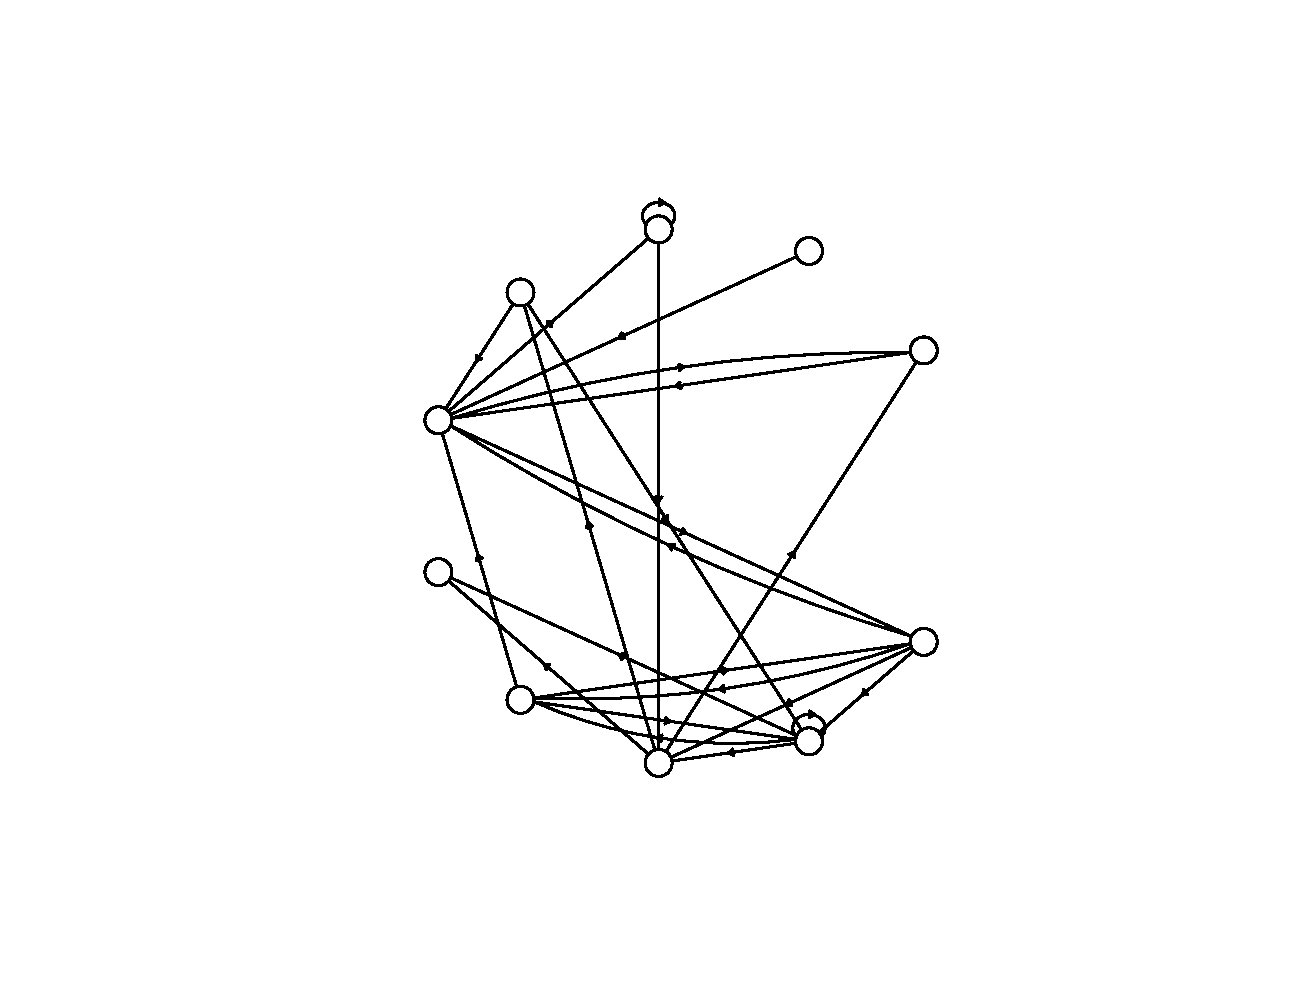
\includegraphics[width=0.8\textwidth]{q2.eps}
    \caption{Graphe considéré.}
\end{figure}

\paragraph*{Question 3.} On a :

\begin{align*}
	P &= \alpha P_1 + (1 - \alpha) e z \\
	\text{o\`u } P_1 &= P_{ss} + dz \\
	\text{donc } P &= \alpha P_{ss} + \alpha (d - e) z + e z
\end{align*}

On peut alors décomposer le calcul comme suit :

\begin{align*}
P^T x
&= (\alpha P_{ss} + \alpha ((d - e) z + ez)^T x \\
&= \alpha P_{ss}^T x + \alpha z^T (d - e)^T x + z^T e^T x \\
&= \alpha P_{ss}^T x + z^T (\alpha (d - e) + e)^T x \\
&= \alpha P_{ss}^T x + z^T w x \\
\end{align*}

Avec $w = (\alpha (d - e) + e)^T$. Le caractère creux des opérations est conservé.

\paragraph*{Question 4.}
~
\begin{lstlisting}
// pi^T est un vecteur propre de P^T associe a la valeur propre 1
[R, diagevals]=spec(P');
index = find(abs(diag(diagevals - 1)) < 1.e-10); // indices dans la liste R des vecteurs propres associes a la valeur propre 1
pi = real(R(:, index))';
pi = pi / sum(pi);
\end{lstlisting}
% dessiner le graphe

On trouve $\pi$ et on vérifie que $\pi^T$ est bien vecteur propre de $P^T$.

\begin{figure}[H]
    \centering
    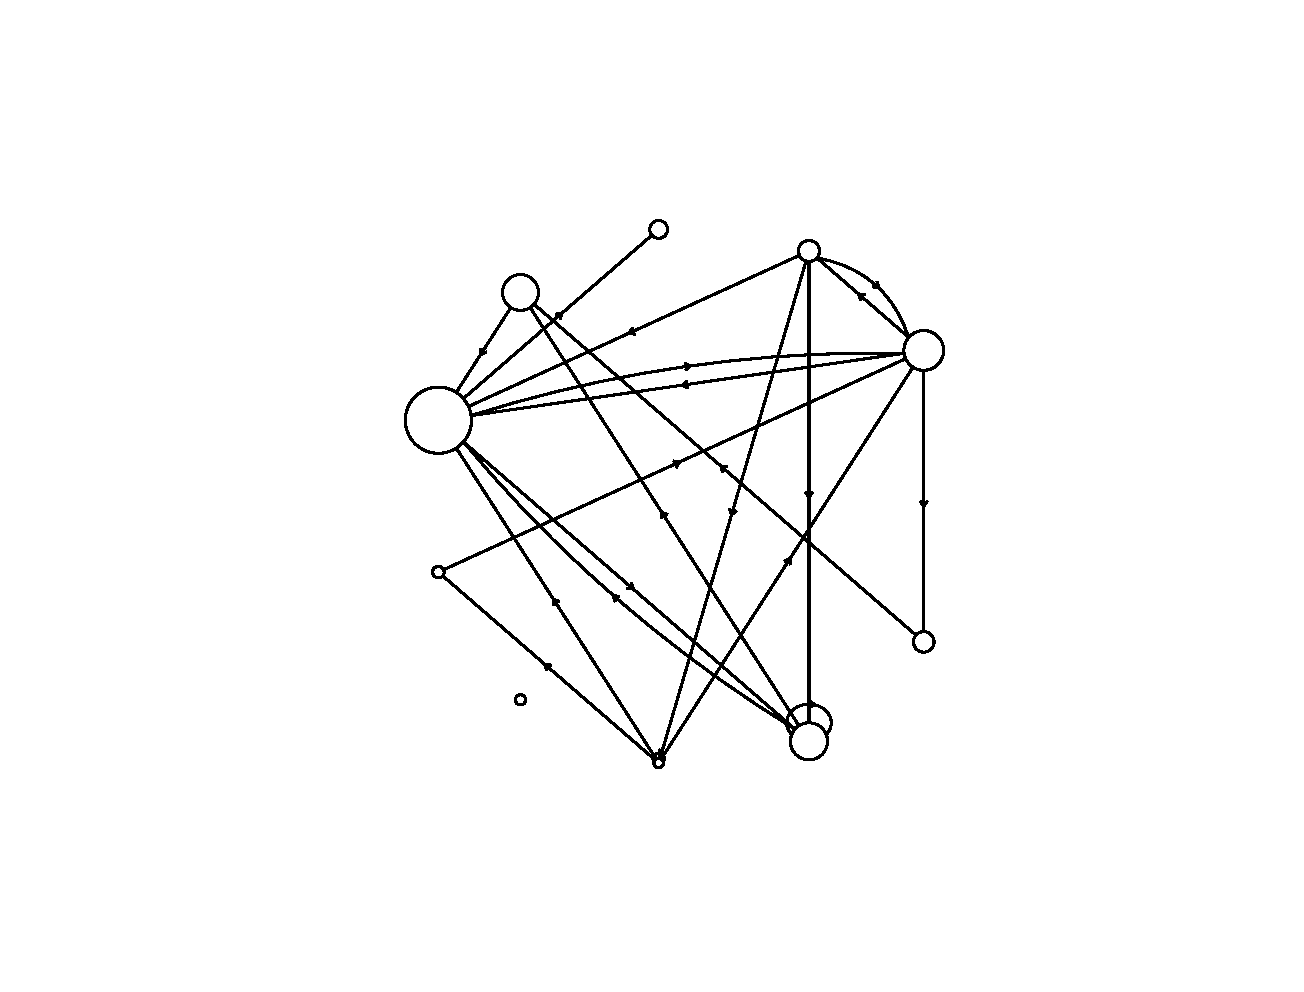
\includegraphics[width=0.8\textwidth]{q4.eps}
    \caption{Graphe en tenant compte du PageRank pour choisir le diamètre du cercle représentant chaque noeud.}
\end{figure}

\paragraph*{Question 5.}
~
\begin{lstlisting}
function [pi]=pi_iterative(P)
  p = ones(n, 1);
  while %t
    pn = P' * p;
    if norm(pn - p, %inf) < 10 * %eps then break;end
    p = pn;
  end
  pi = p';
  pi = pi / sum(pi);
endfunction
\end{lstlisting}

On retrouve le $\pi$ de la question précédente et on vérifie de même que $\pi^T$ est bien vecteur propre de $P^T$.

\paragraph*{Question 6.}
~
\begin{lstlisting}
function [pi]=pi_iterative_sparse(Pss, d, z, alpha)
  p = ones(n, 1);
  while %t
    w = (alpha * (d - ones(n, 1)) + ones(n, 1))';
    pn = alpha * Pss' * p + z' * (w * p);
    if norm(pn - p, %inf) < 10 * %eps then break; end
    p = pn;
  end
  pi = p';
  pi = pi / sum(pi);
endfunction
\end{lstlisting}

On trouve de même $\pi$.

\paragraph*{Question 7.}
%TODO

\paragraph*{Question 8.}
~
\begin{lstlisting}
function cerg=ergodique_markov_T(T,P)
  Pk = eye(n,n);
  couts = r((1:n)');
  cerg = couts;
  for i = 1:T
    Pk = P * Pk;
    cerg = cerg + Pk * couts;
  end
  cerg = cerg / T;
endfunction
\end{lstlisting}

On trouve, pour T = 100 000, $\begin{pmatrix} 6.7799461 \\ 6.7799801 \\ 6.780027 \\ 6.7801198 \end{pmatrix}$.

\begin{lstlisting}
    function [cerg,pi]=ergodique_markov(P)
      pi = pi_iterative(P);
      couts = r((1:n)');
      cerg = pi * couts;
    endfunction
\end{lstlisting}

On trouve 6.779941, soit un écart relatif d'au plus $4 \times 10^{-6}$.

\paragraph*{Question 9.}
On vérifie bien toutes les relations présentées dans le sujet.

\paragraph*{Question 10.}
On suppose que $w$ est un point fixe de $w \mapsto \alpha P_1 w + b$. $w$ vérifie donc $w = \alpha P_1 w + R$, en remarquant que $b = R$.

On a donc :
\begin{align*}
    w + c e &= \alpha P_1 w + R + (1 - \alpha) z w e\\
    &= (\alpha P_1 + (1 - \alpha) e z)w + R \\
    &= P w + R
\end{align*}

Car $zw$ est un scalaire donc commute avec $e$.

\paragraph*{Question 11.}
On montre que l'opérateur $w \mapsto \alpha P_1 w + b$ est contractant. En effet, la norme triple d'une matrice stochastique vaut 1, et on a pris $\alpha = 0.8$.

Ainsi, en vertu du théorème de point fixe de Picard, cet opérateur possède un unique point fixe, et il peut être calculé par itérés.

\end{document}
